{\color{solution}
\begin{enumerate}
	\item $~~\textcolor{exampoints}{(2P)}~~L:\mathbb{F}^n\rightarrow[0,+\infty)$ norm: $\Leftrightarrow$
	\begin{align*}
	&\text{i)}~L(x)=0~~\Rightarrow~~x=0\\
	&\text{ii)}~L(\lambda x)=|\lambda|L(x)\\
	&\text{iii)}~L(x+y)\leq L(x)+L(y)
	\end{align*}
	%
	\item 
	$A=U\Sigma V^T=\sum_{j=1}^{\text{min}(n,m)}\sigma_ju_jv_j^T$\\
	best rank-k approximation is given by truncated SVD
	\begin{align*}
	&\textcolor{exampoints}{(1P)}~~A_k:=\sum_{j=1}^{k}\sigma_ju_jv_j^T~\text{for which}\\
	&\textcolor{exampoints}{(1P)}~~A_k:=\min_{B,\text{rank}(B)=k}\|B-A\|_F^2.
	\end{align*}
	%
	\item $~~\textcolor{exampoints}{(2P)}~~A=\begin{pmatrix}0&1\\1&1\end{pmatrix}$
	%
	\item $~~\textcolor{exampoints}{(2P)}~~A\in\mathbb{R}^{n\times n}~\text{symmetric}~, \lambda_1\neq\lambda_2\in\sigma(A)~\text{with}~v_1, v_2$
	\begin{align*}
	\Rightarrow~~&v_1^TAv_2=\lambda_2v_1^Tv_2\\
	\text{and}~~&v_1^TAv_2=v_2^TA^Tv_1=\lambda_1v_1^Tv_2\\
	\Rightarrow~~&(\lambda_1-\lambda_2)v_1^Tv_2=0\\
	\stackrel{\textcolor{blue}{\lambda_1\neq\lambda_2}}{\Rightarrow}~~&v_1^Tv_2=0
	\end{align*}
	%
	\item 
	$A\in\mathbb{R}^{n\times n}$ positive definite $:\Leftrightarrow~~\forall x\in\mathbb{R}^n\setminus\{0\}:~x^TAx>0$
	\begin{align*}
	&\Rightarrow~~0<x^T\underbrace{(Ax)}_{\textcolor{blue}{:=z}}=\text{cos}(\alpha)\underbrace{\|x\|\|Ax\|}_{\textcolor{blue}{\geq 0}}~~\textcolor{exampoints}{(1P)}\\
	&\Rightarrow~~\text{cos}(\alpha)>0~~\Rightarrow~~\alpha\in\left(-\frac{\pi}{2},\frac{\pi}{2}\right),~|\alpha|<90^{\text{o}}~~\textcolor{exampoints}{(1P)}
	\end{align*}
	%
	\item $~~\textcolor{exampoints}{(1P)}~~f:X\rightarrow Y~\text{injective}~~:\Leftrightarrow~~f(x)=f(y)~~\Rightarrow~~x=y~~\forall x,y\in X$
	%
	\item $P:\mathbb{R}^n\times\mathbb{R}^n\rightarrow \mathbb{R}$ scalar product, if
	\begin{align*}
	&\textcolor{exampoints}{(1P)}~~\text{i)}~~\forall x,y\in\mathbb{R}^n:~P(x,y)=P(y,x)\\
	&\textcolor{exampoints}{(1P)}~~\text{ii)}~~\forall x\in\mathbb{R}^n\setminus\{0\}:~P(x,x)>0\\
	&\textcolor{exampoints}{(1P)}~~\text{iii)}~~\forall x,y,z\in\mathbb{R}^n:~P(x,y+z)=P(x,y)+P(x,z)\\
	&\textcolor{exampoints}{(1P)}~~\text{iv)}~~\forall x,y\in\mathbb{R}^n,\lambda\in\mathbb{R}:~P(x,\lambda y)=\lambda P(x,y)
	\end{align*}
	%
	\item 
	\begin{itemize}
		\item 
		$\textcolor{exampoints}{(1P)}$ pseudoinverse: $A^+=V\Sigma^+U^T$, where $\Sigma^+=\text{diag}(\frac{1}{\sigma_i}:~\sigma_i\neq 0)$
		\item 
		Let $A\in GL_n(\mathbb{R})$, then $\textcolor{exampoints}{(1P)}~\sigma_{ii}\neq 0~\forall i$ and $A^{-1}=(U\Sigma V^T)^{-1}=V\Sigma^{-1}U^T~\textcolor{exampoints}{(1P)}~\\
		(V,U~\text{orthogonal})$. Since $\Sigma^{-1}=~\text{diag}(\frac{1}{\sigma_i})=\Sigma^+$ we find $A^{-1}=A^+~~\textcolor{exampoints}{(1P)}$
	\end{itemize}
	%
	\item 
	%
	\item 
	%
	\item $~~\textcolor{exampoints}{(1P)}~~\mathbb{R}^{m\times n},~~P_n(\mathbb{R}):=\{x\mapsto\sum_{i=0}^{n}\alpha_ix^i:~(\alpha_0,\dots,\alpha_n)\in\mathbb{R}^{n+1}\}$
	%
	\item 
	$\{v_1,\dots,v_n\}\subset V$ basis :$\Leftrightarrow$
	\begin{align*}
	&\textcolor{exampoints}{(1P)}~~\text{i)}~~\{v_1,\dots,v_n\}~\text{linearly independent}~~(\Leftrightarrow~\sum \lambda_jv_j=0~\Rightarrow~\lambda_j=0~\forall~j\\
	&\textcolor{exampoints}{(1P)}~~\text{ii)}~~\text{span}(v_1,\dots,v_n)=V~~\textcolor{blue}{(\Leftrightarrow~\{\sum \lambda_jv_j:~\lambda_j\in\mathbb{R}\}=V)}
	\end{align*}
	%
	\item 
	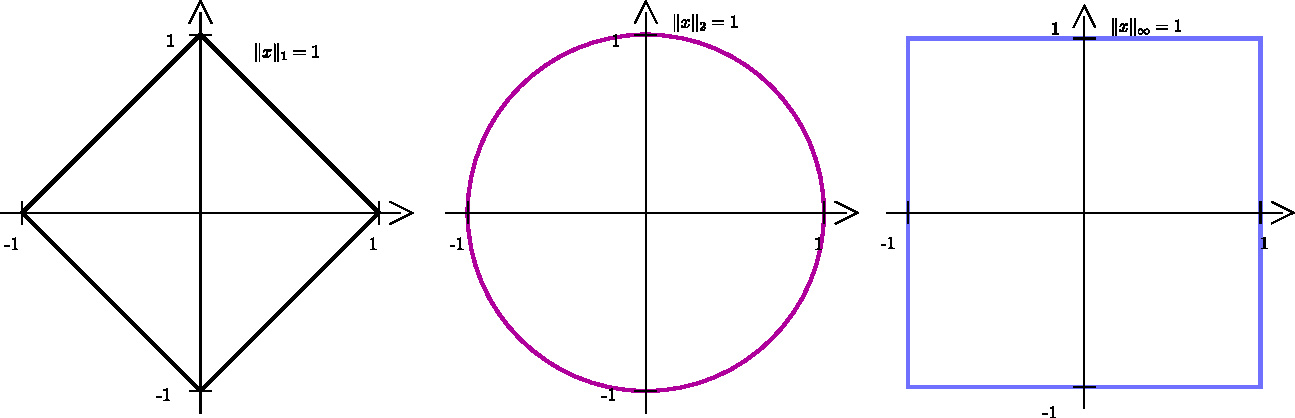
\includegraphics[width=0.25\textwidth]{norms.pdf}	
	\item 
	$\textcolor{exampoints}{(2P)}~$ The power iteration is an algorithm to find an eigenvector of a matrix\\ $A\in\mathbb{R}^{n\times n}$ corresponding to its largest eigenvalue. 
	The drawback of this algorithm is the previous mentioned fact, that the resulting eigenvector is corresponded to the largest eigenvalue.\\
	The iterations are computed by $x^{k+1}:=\frac{Ax^k}{\|Ax^k\|}$.\\
	As an alternative you can use the Inverse Power iteration.
	%
	\item 
	$\textcolor{exampoints}{(2P)}~$ $R$ is not invertible, because triangular matrices are invertible if and only if all diagonal entries are nonzero (see backward/forward substitution)
	%
	\item 
	$\textcolor{exampoints}{(2P)}~$ No!
	\begin{align*}
	&\lambda_i\in\sigma(A^TA),~\sigma_i:=\sqrt{\lambda}=|\tilde{\lambda}_i|\\
	&\tilde{\lambda}_i\in\sigma(A)~~\Rightarrow~~\tilde{\lambda}_i=\lambda_i\in\sigma(A^TA)=\sigma(A^2)
	\end{align*}
	\underline{Thus:} They are only equal up to the sign.
	%
	\item 
	$\textcolor{exampoints}{(2P)}~$ Insert $A=QR$ into the normal equation:
	\begin{align*}
	A^TAx=A^Tb~~&\Leftrightarrow~~(QR)^TQRx=(QR)^Tb~~\Leftrightarrow~~R^TRx=R^TQ^Tb\\
	&\stackrel{\textcolor{blue}{[R^T~\text{invertible, since A has independent columns}]}}{\Leftrightarrow}Rx=Q^Tb
	\end{align*}
	%
	\item $\textcolor{exampoints}{(2P)}~$ The rank of a real matrix $A\in\mathbb{R}^{n\times m}$ is defined as the number of positive singular values ($=\text{dim}(\text{Im}A)~=$ number of linear independent columns).
	%
	\item $\textcolor{exampoints}{(2P)}~\text{rank}(A)+\text{dim}(\text{ker}(A))=n~~(\text{for}~A\in\mathbb{R}^{m\times n})$
	%
	\item 
	$\textcolor{exampoints}{(2P)}~A\in\mathbb{R}^{m\times n}$, then the first k principal components are given by
	$$
	U_k:=\begin{matrix}\text{argmin}\\
	{z\in\mathbb{R}^{m\times k}~\text{\tiny{orthogonal}}}\end{matrix}~\|A-zz^TA\|_{F}^2.
	$$	
	%
	\item $\textcolor{exampoints}{(1P)}~~D=~\text{diag}(d_{ii})$ invertible $\Leftrightarrow~~d_{ii}\neq 0~\forall i$\\
	$\textcolor{exampoints}{(1P)}$ Then $D^{-1}=~\text{diag}(\frac{1}{d_{ii}})$
	%
	\item 
	$\textcolor{exampoints}{(1P)}$ Purpose: Compute eigenvalues of a matrix $A\in\mathbb{R}^{n\times n}$
	\begin{align*}
	\textcolor{exampoints}{(1P)}~~A_0&:=A\\
	\text{for}~&i=1,\dots,n\\
	&Q_iR_i:=A_i\\
	&A_{i+1}:=R_iQ_i
	\end{align*}
	%
	\item $\rho(M)<1~\textcolor{exampoints}{(1P)}~~\Rightarrow~~(x_k)_k$ converges to fixed point $x^*=Mx^*+b~~\textcolor{exampoints}{(1P)}$
	%
	\item $\textcolor{exampoints}{(1P)}~~Q\in\mathbb{R}^{n\times n}$ orthogonal $:\Leftrightarrow~~Q^TQ=I$\\
	$\textcolor{exampoints}{(1P)}$ 
	Thus the columns of $Q$ are mutually orthonormal.
\end{enumerate}
}
\begin{enumerate}
	\item 
	$\textcolor{exampoints}{(2P)}~$ The rank of a real matrix $A\in\mathbb{R}^{n\times m}$ is defined as the number of positive singular values ($=\text{dim}(\text{Im}A)~=$ number of linear independent columns).
	
	\item 
	$\textcolor{exampoints}{(2P)}~$ The power iteration is an algorithm to find an eigenvector of a matrix\\ $A\in\mathbb{R}^{n\times n}$ corresponding to its largest eigenvalue. 
	The drawback of this algorithm is the previous mentioned fact, that the resulting eigenvector is corresponded to the largest eigenvalue.\\
	The iterations are computed by $x^{k+1}:=\frac{Ax^k}{\|Ax^k\|}$.\\
	As an alternative you can use the Inverse Power iteration.
	
	\item 
	$\textcolor{exampoints}{(2P)}~A=\begin{pmatrix}0&1\\1&1\end{pmatrix}$
	
	\item $\textcolor{exampoints}{(2P)}~\text{rank}(A)+\text{dim}(\text{ker}(A))=n~~(\text{for}~A\in\mathbb{R}^{m\times n})$
	
	\item 
	$\textcolor{exampoints}{(2P)}~$ No!
	\begin{align*}
	&\lambda_i\in\sigma(A^TA),~\sigma_i:=\sqrt{\lambda}=|\tilde{\lambda}_i|\\
	&\tilde{\lambda}_i\in\sigma(A)~~\Rightarrow~~\tilde{\lambda}_i=\lambda_i\in\sigma(A^TA)=\sigma(A^2)
	\end{align*}
	\underline{Thus:} They are only equal up to the sign.
	
	\item 
	$\textcolor{exampoints}{(2P)}~A\in\mathbb{R}^{m\times n}$, then the first k principal components are given by
	$$
	U_k:=\begin{matrix}\text{argmin}\\
	{z\in\mathbb{R}^{m\times k}~\text{\tiny{orthogonal}}}\end{matrix}~\|A-zz^TA\|_{F}^2.
	$$
	
	\item 
	$\textcolor{exampoints}{(2P)}~A\in\mathbb{R}^{n\times n}~ \text{positive definite}~~\Rightarrow~~\forall x\neq 0:~x^T\underbrace{Ax}_{\textcolor{blue}{:=z}}>0$ 
	\begin{align*} 
	0<x^Tz =\underbrace{\text{cos}(\alpha)}_{\textcolor{blue}{>0}}\underbrace{\|x\|\|z\|}_{\textcolor{blue}{>0}}~~&\Rightarrow~~\text{cos}(\alpha)>0\\
	&\Rightarrow~~\alpha\in\left(-\frac{\pi}{2},\frac{\pi}{2}\right),~|\alpha|<90^\text{o}
	\end{align*}
\end{enumerate}